\chapter{Исследовательская часть}

\section{Технические характеристики}

Технические характеристики устройства, на котором выполнялся замерный эксперимент:
\begin{itemize}[label*=---]
	\item операционная система Ubuntu 22.04.1 LTS Linux x86\_64 \cite{ubuntu};
	\item память 8 ГБ;
	\item процессор Intel® Core™ i3-7130U;
	\item количество ядер -- 4, количество логических ядер -- 8.
\end{itemize}

Замеры проводилось на ноутбуке, включенном в сеть электропитания. Во время тестирования ноутбук был нагружен только встроенными приложениями окружения, окружением, а также непосредственно замерным экспериментом.

\section{Пример работы программы}

На рисунке \ref{img:example} представлен пример работы программы. Вводится количество вершин в графе и матрица смежности. Далее выводится матрица кратчайших путей и время выполнения последовательного и параллельного алгоритма в микросекундах. Граф из данного примера изображен на рисунке~\ref{img:exampleGraph}. Также при компиляции программы можно указать вывод графа на экран.

\begin{figure}[H]
	\centering
	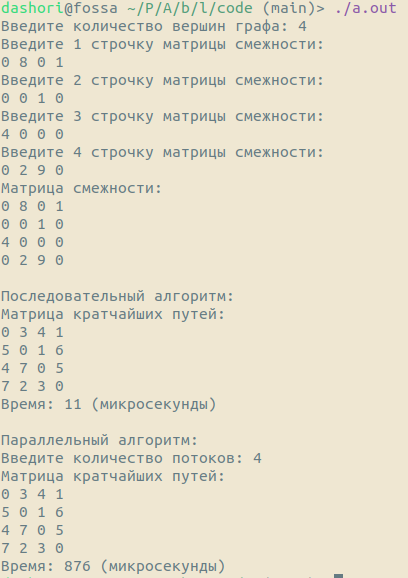
\includegraphics[width=130mm]{images/example}
	\caption{Пример работы программы}
	\label{img:example}
\end{figure}
\begin{figure}[H]
	\centering
	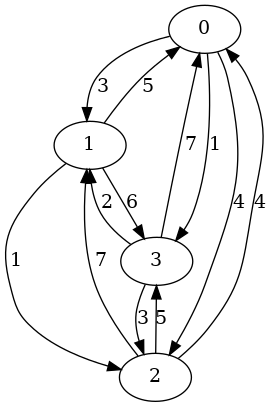
\includegraphics[width=60mm]{images/exampleGraph.png}
	\caption{Пример графа из тестовой программы}
	\label{img:exampleGraph}
\end{figure}

\section{Время выполнения реализованных алгоритмов}

Было проведено два эксперимента по замеру времени. Первый -- зависимость времени работы реализованных алгоритмов от количества потоков, при этом количество вершин графа фиксированно и равно 150. Второй -- зависимость времени  от количества вершин графа, при этом для параллельной реализации алгоритма количество потоков фиксировано и равно 4.

Замеры времени работы реализованных алгоритмов для каждого эксперимента проводились 200 раз. 
В таблице \ref{tab:time} представлен результат зависимости времени работы реализованных алгоритмов от количества вершин в графе, количество потоков для параллельной реализации равно 4. В таблице \ref{tab:timeParallel} представлен результат зависимости времени работы реализованных алгоритмов от количества потоков, количество вершин графа равно 150.
\clearpage
\begin{table}[H]
	\begin{center}
		\begin{flushleft}
			\caption{\label{tab:time}Результаты замеров времени реализованных алгоритмов в микросекундах}
		\end{flushleft}
		\begin{tabular}{|l|l|l|l|l|}
			\hline \specialcell{Количество вершин\\в графе} & \specialcell{Последовательный\\алгоритм} &
			\specialcell{Параллельный\\алгоритм}  \\\hline
			1   & 1      & 428   \\ \hline
			11  & 99     & 162   \\ \hline
			21  & 548    & 617   \\ \hline
			31  & 1467   & 963   \\ \hline
			41  & 3401   & 1805   \\ \hline
			50  & 5831   & 3273   \\ \hline
			100 & 42865  & 20937   \\ \hline
			150 & 138661 & 67138   \\ \hline
			200 & 331876 & 156506     \\ \hline
		\end{tabular}
	\end{center}
\end{table}
\begin{table}[H]
	\begin{center}
		\begin{flushleft}
			\caption{\label{tab:timeParallel}Результаты замеров времени реализованных алгоритмов в микросекундах}
		\end{flushleft}
		\begin{tabular}{|l|l|l|l|l|}
			\hline \specialcell{Количество потоков} & \specialcell{Последовательный\\алгоритм} &
			\specialcell{Параллельный\\алгоритм}  \\\hline
			1  & 137489  & 132363 \\ \hline
			2  & 274394  & 203034 \\ \hline
			3  & 411187  & 284118 \\ \hline
			4  & 546128  & 349896 \\ \hline
			5  & 681251  & 420196 \\ \hline
			6  & 815748  & 488302 \\ \hline
			7  & 950798  & 555731 \\ \hline
			8  & 1094473 &  625521 \\ \hline
			10 & 1367051 & 760079 \\ \hline
			11 & 1502139 & 826971 \\ \hline
			12 & 1637389 & 893409 \\ \hline
			13 & 1772377 & 960084 \\ \hline
			14 & 1907026 & 1028013 \\ \hline
			15 & 2042003 & 1093619  \\ \hline
			16 & 2176615 & 1160360  \\ \hline
		\end{tabular}
	\end{center}
\end{table}

На рисунке \ref{img:result} представлена зависимость времени работы реализованных алгоритмов от количества вершин в графе. На рисунке \ref{img:resultParallel} представлена зависимость времени работы реализованных алгоритмов Флойда от количества потоков.

\begin{figure}[H]
	\centering
	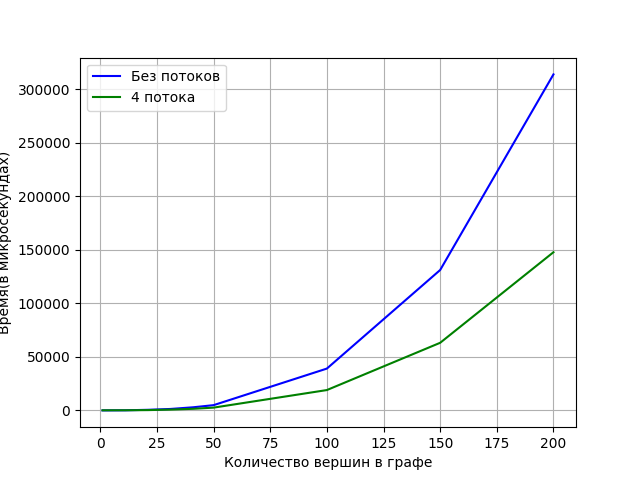
\includegraphics[width=140mm]{images/result}
	\caption{Зависимость времени работы реализованных алгоритмов Флойда от количества вершин в графе}
	\label{img:result}
\end{figure}
\begin{figure}[H]
	\centering
	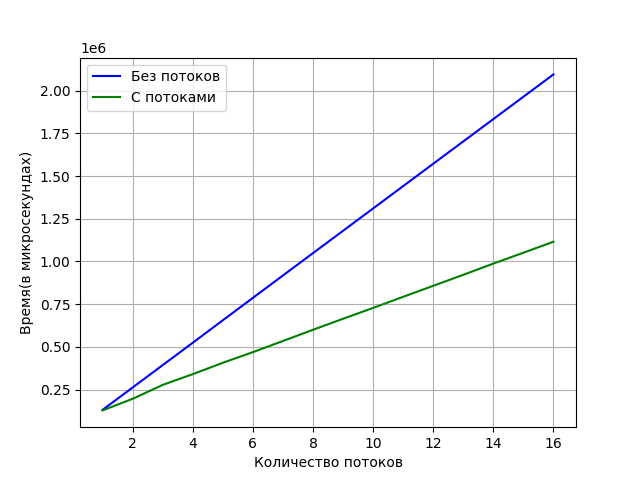
\includegraphics[width=140mm]{images/resultParallel}
	\caption{Зависимость времени работы реализованных алгоритмов Флойда от количества потоков при фиксированном количестве вершин графа}
	\label{img:resultParallel}
\end{figure}

\clearpage
Реализация параллельного алгоритма Флойда превосходит последовательную реализацию в 1.35 раз на двух потоках и в 1.87 раз при восьми потоках. Данный эксперимент проводился на графе с количеством вершин 150 и показывает разницу во времени между параллельной и последовательной реализации, которая зависит от количества потоков.

При сравнении работы реализованных алгоритмов от количества вершин графа было зафиксированно 4 потока. Параллельная реализация алгоритма Флойда выигрывает последовательную реализацию, когда количество вершин графа превышает 30. Если в графе 200 вершин, то параллельная реализация превосходит последовательную в 2.2 раза.
